
%---------------------- chap 1 ----------------------
\cchapter{مقدمه}
\pagebreak

بر اساس آمارهای سازمان سلامت جهانی\LTRfootnote {World Health Organization} بیماری‌های قلبی-عروقی \LTRfootnote{Cardiovascular diseases} رتبه‌ی اول را در بین بیماری‌های کشنده در سطح جهان دارند. برای مثال در سال ۲۰۱۶ حدود ۱۷/۹ میلیون مرگ (حدود ۳۱٪ آمار کلی فوت) به علت بیماری‌های قلبی عروقی تخمین زده شده‌است. \cite{WHO} حدود ۲۵٪ این تعداد را مرگ‌های ناگهانی قلبی (SCD) تشکیل می‌دهند. \cite{Srinivasan2018} در چنین شرایطی، بیمار در طول مدت یک ساعت پس از آغاز علایم دچار ایست قلبی می‌شود. 
علت اصلی ایست‌های قلبی ناگهانی، آریتمی‌های قلبی هستند. \cite{Cleveland} این عبارت به دسته‌ای از بیماری‌های قلبی اطلاق می‌شود که در آن‌ها، اختلالاتی در آهنگ طبیعی تپش قلب به وجود می‌آید. با وجود این که بیشتر آریتمی‌ها بی خطر هستند، در برخی موارد در صورت عدم رسیدگی می‌توانند مرگبار باشند. به همین دلیل، تشخیص و درمان به موقع آن‌ها از اهمیت بالایی برخوردار است. 

یکی از رایج‌ترین و مهم‌ترین ابزارها در تشخیص بیماری‌های قلبی-عروقی، سیگنال نوار قلب \LTRfootnote{Electrocardiogram (ECG)} است. \cite {Elgendi2014} قلب ماهیچه‌ای است که با تحریک سیگنال‌های الکتریکی، به صورت منظم در حال تپش است. این فعالیت الکتریکی قلب، باعث ایجاد نوساناتی متناوب در پتانسیل الکتریکی سطح پوست می‌شود. این نوسانات  را می‌توان به کمک الکترودهایی که روی پوست قرارمی‌گیرند، اندازه‌گیری و در قالب سیگنال نوار قلب ثبت نمود. 

تحلیل سیگنال نوار قلب، اطلاعات مفیدی در راستای تشخیص آریتمی و نوع آن فراهم می‌کند. \cite{Mondejar} از همین روی، در چند دهه‌ی گذشته پژوهش‌های گسترده‌ای بر روی طراحی سیستم‌های خودکار تشخیص آریتمی صورت گرفته‌است. در این سیستم‌ها، ابتدا سیگنال نوار قلب به وسیله‌ی الکترودها و تجهیزات مخصوص، از بیمار گرفته شده و فیلترهایی به جهت حذف انواع نویزها بر روی آن اعمال می‌شود. قدم بعدی، استخراج تک‌تک ضربان‌های یک سیگنال نوار قلب است. در این مرحله یک الگوریتم قطعه‌بندی \LTRfootnote{Segmentation} بر روی نوار قلب اجرا می‌شود.

هر تک‌ضربان قلب شامل تعدادی موج است که در کنار هم نوسانات ضربان را تشکیل می‌دهند. موج‌های \lr{Q}، \lr{R} و \lr{S} مهم‌ترین موج‌ها در تحلیل نوار قلب هستند.\cite{Mondejar} به مجموعه‌ی این سه موج در کنار هم، ترکیب \lr{QRS} گفته می‌شود. به دلیل اهمیت این ترکیب در تشخیص انواع آریتمی، بخش مهمی از کارهای گذشته به تشخیص خودکار این ترکیب در ضربان قلب اختصاص داده شده‌است. معمولا در مرحله‌ی قطعه‌بندی موقعیت زمانی ترکیب \lr{QRS} هر ضربان و یا قله‌های \lr{R} در ضربان‌های متوالی تشخیص داده می‌شود.

 در مرحله‌ی بعد، مجموعه‌ای از ویژگی‌ها از هر یک از ضربان‌ها استخراج شده و به یک دسته‌بند \LTRfootnote{Classifier} داده‌می‌شود. این دسته‌بند نوع ضربان که خروجی نهایی این سیستم است را تعیین می‌کند. دیاگرام معماری کلی چنین سیستمی در شکل \ref{classifierPicture} قابل مشاهده است. 
 
\begin{figure}[!htb]
\centering
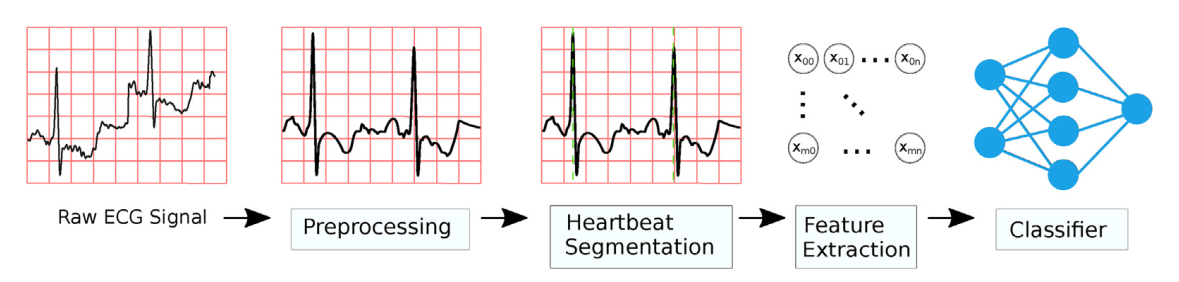
\includegraphics[width=15cm]{Figures/classifier.png}
\caption{مراحل اصلی یک سیستم خودکار تشخیص آریتمی\cite{Mondejar}}
\label{fig:classifierPicture}
\end{figure}

در این پروژه، هدف بر این است که بستری بی‌درنگ برای تشخیص آریتمی فراهم شود. به دلیل اهمیت تشخیص سریع در برخی از انواع خطرناک آریتمی، به خصوص آریتمی‌هایی که منجر به ایست ناگهانی قلبی می‌شوند، بی‌درنگ بودن این سیستم حایز اهمیت است. این امر نیازمند این است که تمامی بخش‌های سیستم، شامل بخش پیش‌پردازش،‌ بخش استخراج ویژگی و الگوریتم دسته‌بندی، همگی توانایی کارکردن به صورت برخط را داشته‌باشند. به بیان دیگر این سیستم به شکل خط‌لوله‌ای طراحی شده‌است که در آن ضربان‌ها به صورت پی‌در‌پی تولید، پردازش‌ و دسته‌بندی می‌شوند. پس از پیاده‌سازی، تاخیر هر یک از بخش‌ها اندازه‌گیری شده و تاخیر کلی سیستم تخمین زده می‌شود. 
همان‌طور که گفته‌شد، اولین بخش سیستم، بخش پیش‌پردازش ضربان قلب است. در این بخش یک الگوریتم تشخیص QRS طبق روش پن و تامپکینز (منبع)  پیاده‌سازی شده‌است. این الگوریتم یک روش بی‌درنگ است که سیگنال دیجیتال‌شده‌ی نوار قلب را به عنوان ورودی دریافت کرده و موقعیت زمانی قله‌های R را در هر یک از ضربان‌ها تشخیص می‌دهد. فاصله‌ی هر قله‌ی R تشخیص‌داده‌شده با قله‌ی بعدی و قبلی خود، که تحت عنوان فاصله‌ی R-R شناخته می‌شود، مهم‌ترین ویژگی در تشخیص نوع ضربان قلب (نوع آریتمی آن ضربان) است. (نیازمند منبع) 
در مرحله‌ی بعد، ویژگی‌های مورد نظر، از فواصل R-R تشخیص‌داده‌شده استخراج می‌گردند. این ویژگی‌ها سپس به یک دسته‌بند SVM که پیش‌تر مراحل یادگیری را طی کرده‌است، داده می‌شوند و دسته‌بند به کمک ویژگی‌های ورودی، نوع آریتمی را تشخیص می‌دهد. ضربان‌های دارای آریتمی انواع متعددی دارند که در ۵ دسته‌ی کلی دسته‌بندی می‌شوند. خروجی سیستم ما، تشخیص یکی از این دسته‌ها برای هر ضربان قلب است.

یکی از نیازمندی‌های بستر طراحی‌شده در این پروژه، این است که بتوان سیستمی قابل حمل و قابل استفاده‌ی آسان برای بیمار را بر روی این بستر پیاده‌سازی کرد. برای پیاده‌سازی این کاربرد، اینترنت اشیا راه‌حل مناسبی تشخیص داده‌شد. در چنین کاربردی، انتظار می‌رود بیمار دستگاهی ساده در اختیار داشته‌باشد که ضربان قلب او را دریافت کرده و پیش‌پردازش‌هایی ساده را بر روی آن پیاده نماید، و پردازش‌های پیچیده‌تر برای تشخیص آریتمی، بر عهده‌ی یک سرور با توان پردازشی بالاتری باشد. سپس نتایج این پردازش‌ها به اطلاع بیمار و پزشک او برسد.

 برای این منظور، معماری کلی سیستم به دو بخش تقسیم شد. بخش اول سیستم، وظیفه‌ی دریافت ضربان قلب از بیمار،‌ انجام پیش‌پردازش‌هایی بر روی آن، و در انتها ارسال نتایج پیش‌پردازش به سرور را دارد. این بخش به صورت سخت‌افزاری پیاده شده‌است و کافی است یک حس‌گر دیجیتال ضربان قلب، برای دریافت ضربان قلب بیمار به آن متصل شود. 
بخش دوم سیستم با استفاده از الگوریتم‌های یادگیری ماشین، و بر روی یک سرور پیاده‌سازی شده‌است. در این سرور، نتایج پیش‌پردازش‌های انجام شده در بخش قبل در سرور دریافت شده و ویژگی‌های هر ضربان استخراج می‌شود. سپس با استفاده از این ویژگی‌ها، عمل دسته‌بندی ضربان‌ها انجام می‌شود.

کارهای گذشته در قسمت فیچر:
در کارهای گذشته، ویژگی‌های مختلفی برای توصیف ضربان قلب معرفی شده‌اند. تبدیل موجک (منبع) و آمارهای مرتبه بالاتر (HOS) (منبع) از جمله‌ی این ویژگی‌ها هستند. در تبدیل موجک، اطلاعاتی هم در حوزه‌ی زمان و هم در حوزه‌ی فرکانس از سیگنال استخراج می‌شود. 
(توضیحات بیشتر در مورد اینترنت اشیا)
در برخی از پژوهش‌ها از بازه‌های R-R به عنوان ویژگی استفاده شده‌است (منبع) (منبع ۶۷ تا ۷۹ سوروی). آریتمی قلبی باعث برهم‌خوردن آهنگ تپش و در نتیجه‌ی آن، توازن منحنی ضربان قلب می‌شود، و ابن اتفاق تاثیر مستقیمی بر روی نوسانات فاصله‌های قله‌های R می‌گذارد. (منبع ۱ سوروی) به همین دلیل ویژگی R-R ظرفیت بالایی برای تشخیص انواع آریتمی دارد. این ویژگی در بین ویژگی‌های به کار گرفته‌شده پراستفاده‌ترین است. (منبع ۱۵ مرده خوار)
این ویژگی، نسبت به ویژگی‌های morphological حجم کم‌تری به خود اختصاص می‌دهد. در کار پیش رو، ویژگی‌های استخراج شده از ضربان قلب بیمار در مرحله‌ی پیش‌پردازش، به یک سرور فرستاده می‌شوند تا پردازش‌های بیش‌تر بر روی آن‌ها انجام شود. از این رو لازم است حجم داده‌های ارسال‌شده، و پیرو آن، حجم ویژگی‌های استخراج‌شده کنترل شود. در صورتی که ویژگی‌های استخراج‌شده حجم زیادی داشته‌باشند، تاخیر ارسال آن‌ها به سرور بالا رفته و تاثیری منفی بر روی تاخیر کل سیستم خواهدداشت. با توجه به اهمیت تاخیر پایین و بی‌درنگ بودن عملیات در این کاربرد، و همچنین دقت بالای بازه‌های R-R در تعیین نوع آریتمی، از این ویژگی استفاده کردیم. 
(normalized RR)

قدم بعد، پیاده‌سازی یک دسته‌بند برای تعیین نوع آریتمی است. در کارهای گذشته از الگوریتم‌های دسته‌بندی مانند SVM ANN (از رو مقاله هه بنویس با منبع) استفاده شده‌است. در کار پیش رو، SVM به دلیل کارایی مناسبی که در کارهای گذشته (منبع ۲۱ و ۲۲ مرده خوار) نشان داده‌است به کار گرفته شده‌است. 


